\documentclass[11pt,oneside]{article}
\usepackage[utf8]{inputenc}
\usepackage[a4paper,top=2cm,left=2cm,right=2cm,bottom=2cm]{geometry}
\usepackage{import}
\usepackage[T1]{fontenc}
\usepackage[german,ngerman]{babel}
\usepackage[table]{xcolor}
\usepackage{amsthm, esvect}
\usepackage{mathtools}
\RequirePackage{amssymb, amsfonts, amsmath, latexsym, verbatim, xspace}
\usepackage{systeme}
\usepackage{multicol}
\usepackage{multirow}
\usepackage{framed}
\usepackage{array}
\usepackage{ragged2e}
\usepackage{graphicx}
\usepackage{pdflscape}
\usepackage{epstopdf}
\usepackage{booktabs}
\usepackage{pdfpages}
\usepackage{float} % Allows putting an [H] in \begin{figure} to specify the exact location of the figure
\usepackage{wrapfig} % Allows in-line images such as the example fish picture
\usepackage{tikz, graphicx} % tikz
\usepackage[position=top]{subfig}
\usepackage[bookmarks=true]{hyperref}%Links
\usepackage{enumerate}
\usepackage{enumitem}
\usepackage[german,ruled,vlined,linesnumbered,algosection]{algorithm2e}
\usepackage[labelfont=sf]{caption}
\usepackage{lmodern}
\usepackage{lscape}
\usepackage{tabularx}
\usepackage{systeme}
\usepackage{hhline}
\usepackage{subfiles}
\usepackage{stackengine}
\usepackage{setspace}
\usepackage{MnSymbol}
\usepackage{tcolorbox}
\usepackage{bbm}
\usepackage{url}
\usepackage{xparse}
\usepackage{sectsty}
\usepackage{array}
\usepackage{ragged2e}
\usepackage{listings} %Stellt Code-Snippets sauber dar

% definiert die Sprache
\selectlanguage{German}

% add command for different dates in Swiss fashion
\newcommand{\monthwordlong}[1]{\ifcase#1 \or Januar\or Februar\or März\or April\or Mai\or Juni\or Juli\or August\or September\or Oktober\or November\or Dezember\fi}
\newcommand{\monthwordshort}[1]{\ifcase#1\or Jan\or Feb\or Mar\or Apr\or Mai\or Jun\or Jul\or Aug\or Sept\or Okt\or Nov\or Dez\fi}
\newcommand{\datelong}{\number\day.\:\monthwordlong{\the\month}\:\number\year}
\newcommand{\dateshort}{\number\day.\:\monthwordshort{\the\month}\:\number\year}

% define color of links inside a text
\definecolor{linkblue}{RGB}{0, 0, 80}
\definecolor{plotblue}{RGB}{100, 100, 255}
\definecolor{myblue}{RGB}{8,164,214}
\definecolor{myred}{RGB}{143,42,41}
\definecolor{forestgreen}{RGB}{34,139,34}
\definecolor{highdive}{RGB}{10,169,194}
\definecolor{charcoal}{RGB}{74,74,74}
\hypersetup{
	colorlinks=true,
	linkcolor=linkblue,
	filecolor=magenta,
	urlcolor=plotblue,
	citecolor=linkblue,
	pdfpagemode=FullScreen,
}


\lstdefinestyle{mystyle}{ % definiert den style des Code-Snippets
	%backgroundcolor=\color{backcolour},
	%commentstyle=\color{codegreen},
	%keywordstyle=\color{magenta},
	%numberstyle=\tiny\color{codegray},
	%stringstyle=\color{codepurple},
	basicstyle=\ttfamily\footnotesize,
	breakatwhitespace=false,
	breaklines=true,
	captionpos=b,
	keepspaces=true,
	%numbers=left,
	%numbersep=5pt,
	showspaces=false,
	showstringspaces=false,
	showtabs=false,
	tabsize=4
}
\lstset{style=mystyle}
\usepackage{fancyhdr}

\tcbuselibrary{breakable,skins}
\usetikzlibrary{mindmap,trees}
\newlength\tindent
\setlength{\tindent}{\parindent}
\setlength{\parindent}{0pt}
\renewcommand{\indent}{\hspace*{\tindent}}

\makeatletter
\def\ifEmpty#1{\def\@temp{#1}\ifx\@temp\@empty}
\makeatother

\sectionfont{\underline}
\usetikzlibrary{arrows, petri, topaths, graphs}


% =================== BEISPIEL ====================
\theoremstyle{definition}
\newtheorem{beispiel}{Beispiel}
\renewcommand{\thebeispiel}{\arabic{beispiel}}

% =================== AUFGABE =====================
\newcounter{aufg}[section] % Zähler für die Umgebungen

\newenvironment{aufgabe}[1][]{%
    \refstepcounter{aufg}% Inkrementiere den Zähler
    \begin{tcolorbox}[%
        enhanced,
        overlay unbroken and first={\mytitleaufg[#1]}, % Titelleiste mit Icons wird nicht über Seite gebrochen
        colframe=black,
        boxrule=0pt,
        breakable,
        top=15pt,
        before=\vskip18pt,
    ]
}{%
    \end{tcolorbox}
}

\newcommand{\mytitleaufg}[1][]{% Definiert die Titelleiste und Icons
    \node[fill=black!20,
        rounded corners,
        draw=black,
        text=black,
        line width=1pt,
        inner sep=4pt,
        anchor=west,
        xshift=12pt]
        at (frame.north west){\bfseries Aufgabe \thesection.\theaufg.\ifEmpty{#1}\else\emph{ (#1)}\fi}; % Titel, letzter Teil mit ifempty testet ob #1 leer und macht Klammern und Titel, falls Titelargument übergeben wird bzw. falls #1 leer erscheint nichts - auch keine Klammern

    \node[% Icon
        rounded corners,
        text=black,
        fill=black,
        line width=0pt,
        inner sep=3pt,
        anchor=west,
        xshift=5pt,
        % yshift=-35pt
        ]
        at (frame.north east){
\includegraphics[width=24pt]{../../../Header/Icons/aufgabeicon.png}};
}

% =================== DEFINITION ==================
\newcounter{def}[section] % Zähler für die Umgebungen

\newenvironment{definition}[1][]{%
    \refstepcounter{def}% Inkrementiere den Zähler
    \begin{tcolorbox}[%
        enhanced,
        drop shadow southeast,
        overlay unbroken and first={\mytitledef[#1]}, % Titelleiste mit Icons wird nicht über Seite gebrochen
        colback=blue!5!white,
        colframe=blue!75!black,
        boxrule=2pt,
        breakable,
        top=15pt,
        before=\vskip18pt,
    ]
}{%
    \end{tcolorbox}
}

\newcommand{\mytitledef}[1][]{% Definiert die Titelleiste und Icons
    \node[fill=blue!40!white,
        rounded corners,
        draw=black,
        text=black,
        line width=1pt,
        inner sep=4pt,
        anchor=west,
        xshift=12pt]
        at (frame.north west){\bfseries Definition \thesection.\thedef.\ifEmpty{#1}\else\emph{ (#1)}\fi}; % Titel, letzter Teil mit ifempty testet ob #1 leer und macht Klammern und Titel, falls Titelargument übergeben wird bzw. falls #1 leer erscheint nichts - auch keine Klammern

    \node[% Icon
        rounded corners,
        text=black,
        fill=black,
        line width=0pt,
        inner sep=3pt,
        anchor=west,
        xshift=5pt,
        % yshift=-35pt
        ]
        at (frame.north east){
\includegraphics[width=24pt]{../../../Header/Icons/definitionicon.png}};
}

% =================== NOTATION ====================
\newcounter{nota}[section] % Zähler für die Umgebungen

\newenvironment{notation}[1][]{%
    \refstepcounter{nota}% Inkrementiere den Zähler
    \begin{tcolorbox}[%
        enhanced,
        drop shadow southeast,
        colback=yellow!5!white,
        colframe=yellow!75!black,
        overlay unbroken and first={\mytitlenota[#1]},   % Titelleiste mit Icons wird nicht über Seite gebrochen
        boxrule=2pt,
        breakable,
        top=15pt,
        before=\vskip18pt,
    ]
}{%
    \end{tcolorbox}
}

\newcommand{\mytitlenota}[1][]{% Definiert die Titelleiste und Icons
    \node[fill=yellow!40!white,,
        rounded corners,
        draw=black,
        text=black,
        line width=1pt,
        inner sep=4pt,
        anchor=west,
        xshift=12pt]
        at (frame.north west){\bfseries Notation \thesection.\thenota.\ifEmpty{#1}\else\emph{ (#1)}\fi}; % Titel, letzter Teil mit ifempty testet ob #1 leer und macht Klammern und Titel, falls Titelargument übergeben wird bzw. falls #1 leer erscheint nichts - auch keine Klammern

    \node[% Icon
        rounded corners,
        text=black,
        fill=black,
        line width=0pt,
        inner sep=3pt,
        anchor=west,
        xshift=5pt,
        % yshift=-35pt
        ]
        at (frame.north east){
\includegraphics[width=24pt]{../../../Header/Icons/definitionicon.png}};
}

% =================== SATZ ========================
\newcounter{satz}[section]  % creates a counter and resets it after each chapter

\newenvironment{satz}[1][]{   % Hauptbox mit Satz drin
    \refstepcounter{satz}
    \begin{tcolorbox}[%
        enhanced,
        colback=red!5!white,
        fuzzy halo=2mm with gray,
        colframe=red!75!black,
        overlay unbroken and first={\mytitlesatz[#1]},   % Titelleiste mit Icons wird nicht über Seite gebrochen
        boxrule=2pt,
        breakable,
        top=15pt,
        before=\vskip18pt,
    ]
}{%
    \end{tcolorbox}
}

\newcommand{\mytitlesatz}[1][]{                     % Macht Titelbox und Icons
   \node[fill=red!90!white,
      rounded corners,
      draw=black,,
      text=black,
      line width=1pt,
      inner sep=4pt,
      anchor=west,
      xshift=12pt]
   at (frame.north west){\bfseries Satz \thesection.\thesatz.\ifEmpty{#1}\else\emph{ (#1)}\fi};  % Titel, letzter Teil mit ifx testet ob #1 leer und macht Klammern und Titel, falls Titelargument übergeben wird bzw.  falls #1 leer erscheint nichts - auch keine Klammern

 \node[ % Icon
      rounded corners,
      text=black,
      fill=black,
      line width=0pt,
      inner sep=3pt,
      anchor=west,
      xshift=5pt,
%     yshift=-35pt
]
   at (frame.north east){ 
\includegraphics[width=24pt]{../../../Header/Icons/satzicon.png} };
}

% =================== BEWEIS ======================
\newenvironment{beweis}[1][]{
    \begin{tcolorbox}[
        enhanced,
        overlay unbroken and first={\mybeweis[#1]},     % Titelleiste mit Icons wird nicht über Seite gebrochen
        colback=white,
        colframe=black,
        boxrule=0pt,
        breakable,
        top=15pt,
        before=\vskip18pt,
    ]
}{
        \end{tcolorbox}
}

\newcommand{\mybeweis}[1][]{                     % Macht Titelbox und Icons
   \node[fill=white,
      rounded corners,
      draw=black,
      text=black,
      line width=1pt,
      inner sep=4pt,
      anchor=west,
      xshift=12pt]
   at (frame.north west){\bfseries Beweis \ifEmpty{#1}\else\emph{ (#1)}\fi};  % Titel, letzter Teil mit ifx testet ob #1 leer und macht Klammern und Titel, falls Titelargument übergeben wird bzw.  falls #1 leer erscheint nichts - auch keine Klammern
}

% =================== ALGORITHM ===================
\newcounter{algo}[section]  % creates a counter and resets it after each chapter

\newenvironment{algo}[1][]{   % Hauptbox mit Satz drin
    \refstepcounter{algo}
    \begin{tcolorbox}[%
        enhanced,
        drop shadow southeast,
        colback=yellow!5!white,
        colframe=yellow!75!black,
        overlay unbroken and first={\algotitle[#1]},   % Titelleiste mit Icons wird nicht über Seite gebrochen
        boxrule=2pt,
        breakable,
        top=15pt,
        before=\vskip18pt,
    ]
}{%
    \end{tcolorbox}
}

\newcommand{\algotitle}[1][]{                     % Macht Titelbox und Icons
   \node[fill=yellow!40!white,
      rounded corners,
      draw=black,
      text=black,
      line width=1pt,
      inner sep=4pt,
      anchor=west,
      xshift=12pt]
   at (frame.north west){\bfseries \ifEmpty{#1}{Ablauf}\else{#1}\fi};  % Titel, letzter Teil mit ifx testet ob #1 leer und macht Klammern und Titel, falls Titelargument übergeben wird bzw.  falls #1 leer erscheint nichts - auch keine Klammern

 \node[ % Icon
      rounded corners,
      text=black,
      fill=black,
      line width=0pt,
      inner sep=3pt,
      anchor=west,
      xshift=5pt
      % yshift=-35pt
      ]
   at (frame.north east){ 
\includegraphics[width=24pt]{../../../Header/Icons/algoicon.png} };
}

% ================ Nummerierte Multicol ================
\newenvironment{enumcols}[1][]{
    \begin{enumerate}[label=\alph*)]\begin{multicols}{#1}
}{
    \end{multicols}\end{enumerate}
}



% =================================================
\usetikzlibrary{shapes,arrows}
\tikzstyle{decision} = [diamond, draw, fill=blue!20,
    text width=6em, text badly centered, node distance=4cm, inner sep=0pt]
\tikzstyle{block} = [rectangle, draw, fill=blue!20,
    text width=8em, text centered, rounded corners, minimum height=4em]
\tikzstyle{line} = [draw, -latex']
\tikzstyle{cloud} = [draw, ellipse,fill=red!20, node distance=2cm,
    minimum height=2em]

% Karriertes Papier für Antwort
\newcommand{\karos}[1]{\begin{tikzpicture}\draw[step=0.5cm,color=gray] (0,0) grid (\linewidth,#1 cm);\end{tikzpicture}}
%%
% Header and Footer
%%
\linespread{1.2} % Line spacing
\fancypagestyle{plain}{
	\pagestyle{fancy}
	\lhead{}
	\chead{}
	\rhead{}
	\lfoot{\Autor}
	\cfoot{\Skriptname}
	\rfoot{\thepage}
	\renewcommand{\headrulewidth}{0pt}
	\renewcommand{\footrulewidth}{0.4pt}
}

\pagestyle{fancy}
\fancyhf{}
\rhead{\rightmark}
\lfoot{\leftmark}
\rfoot{\thepage}
\renewcommand{\headrulewidth}{0.2pt}
%\setlength\parindent{0pt} % Uncomment to remove all indentation from paragraphs



%%
% Math Arrows
%%
\newcommand{\same}{\ensuremath{\Longleftrightarrow}}
\renewcommand{\to}{\ensuremath{\longrightarrow}}
\newcommand{\qsame}{\quad\same\quad}
\newcommand{\dsame}{\ensuremath{:\Leftrightarrow}}
\newcommand{\qdsame}{\quad\dsame\quad}
\newcommand{\ldsame}{\ensuremath{:\Longleftrightarrow}}
\newcommand{\samedef}{\ensuremath{\us {\text{def}} \Leftrightarrow}}
\newcommand{\qsamedef}{\quad\samedef\quad}
\newcommand{\lsamedef}{\ensuremath{\us {\text{def}} \Longleftrightarrow}}
\newcommand{\qlsamedef}{\quad\lsamedef\quad}


%%
% Mengendefinitionen
%%
\newcommand{\M}{\ensuremath{\mathcal{M}}}
\newcommand{\N}{\ensuremath{\mathbb{N}}}
\newcommand{\Z}{\ensuremath{\mathbb{Z}}}
\newcommand{\Q}{\ensuremath{\mathbb{Q}}}
\newcommand{\I}{\ensuremath{\mathbb{I}}}
\newcommand{\R}{\ensuremath{\mathbb{R}}}
\newcommand{\C}{\ensuremath{\mathbb{C}}}
\renewcommand{\S}{\ensuremath{\mathbb{S}}}
\newcommand{\Prim}{\ensuremath{\mathbb{P}}}
\newcommand{\0}{\ensuremath{\emptyset}}
\renewcommand{\Re}{\ensuremath{\operatorname{Re}}}
\renewcommand{\Im}{\ensuremath{\operatorname{Im}}}
\newcommand{\strich}{\ensuremath{\big\vert}}

%%
% Mengenoperation
%%
\renewcommand{\nin}{\not\in}


%%
% Logisches Und und Oder
%%
\newcommand{\sand}{\ensuremath{\; \land \;}}
\newcommand{\sor}{\ensuremath{\; \lor \;}}
\renewcommand{\*}{\ensuremath{\cdot}}
\newcommand{\oder}{\vee}
\newcommand{\n}{\neg}
\newcommand{\und}{\wedge}


%%
% Bei Integral, Summe,... die Grenzen über bzw.
% unter das Zeichen
%%
\renewcommand{\d}[1]{\ensuremath{\operatorname{d}\!{#1}}}
\newcommand{\Sum}{\sum\limits}
\newcommand{\Prod}{\prod\limits}
\newcommand{\Min}{\min\limits}
\newcommand{\Max}{\max\limits}
\newcommand{\Lim}{\lim\limits}
\newcommand{\Inf}{\inf\limits}
\newcommand{\Sup}{\sup\limits}
\newcommand{\Liminf}{\liminf\limits}
\newcommand{\Limsup}{\limsup\limits}
%\renewcommand{\Cup}{\bigcup\limits}
%\renewcommand{\Cap}{\bigcap\limits}
\newcommand{\Otimes}{\bigotimes\limits}
\newcommand{\Oplus}{\bigoplus\limits}


%%
% Arcus Cotangens, Logarithmus
%%
\let\oldsin\sin
\renewcommand{\sin}[1]{\oldsin{\left(#1\right)}}
\let\oldcos\cos
\renewcommand{\cos}[1]{\oldcos{\left(#1\right)}}
\let\oldtan\tan
\renewcommand{\tan}[1]{\oldtan{\left(#1\right)}}
\let\oldarcsin\arcsin
\renewcommand{\arcsin}[1]{\oldarcsin{\left(#1\right)}}
\let\oldarccos\arccos
\renewcommand{\arccos}[1]{\oldarccos{\left(#1\right)}}
\let\oldarctan\arctan
\renewcommand{\arctan}[1]{\oldarctan{\left(#1\right)}}
\let\oldln\ln
\renewcommand{\ln}[1]{\oldln{\left(#1\right)}}
\newcommand{\Log}[2]{\ensuremath{\operatorname{log}_{#1}\left(#2\right)}}
\newcommand{\e}{\operatorname{e}}
\renewcommand{\exp}[1]{\ensuremath{\operatorname{\e}^{#1}}}


%%
% Griechische Buchstaben
%%
\renewcommand{\epsilon}{\ensuremath{\varepsilon}}
\renewcommand{\phi}{\varphi}
\renewcommand{\l}{\lambda}
\renewcommand{\t}{\tau}


%%
% Bezeichnungen
%%
\newcommand{\Rgn}{\R_{>0}} % R grösser Null
\newcommand{\Rad}{\operatorname{Rad}}   % Radikal
\newcommand{\kgV}{\operatorname{kgV}}   % Kleinster gemeinsame Vielfache
\newcommand{\ggT}{\operatorname{ggT}}   % Grösster gemeinsame Teiler
\newcommand{\winkel}{\sphericalangle}          % Winkelsymbol
\DeclarePairedDelimiter\abs{\lvert}{\rvert} % besserer Betrag
\makeatletter
\let\oldabs\abs
\def\abs{\@ifstar{\oldabs}{\oldabs*}}
\makeatother


%%
% Vektorgeometrie
%%
\renewcommand{\v}[1]{\vv{#1}}       % besserer Pfeil über Buchstaben
\renewcommand{\vec}[2]{\begingroup\renewcommand{\arraystretch}{1}\left(\begin{array}{c} #1 \\ #2 \end{array}\right)\endgroup}   % two dimensional vector
\renewcommand{\Vec}[3]{\begingroup\renewcommand{\arraystretch}{1}\left(\begin{array}{c} #1 \\ #2 \\ #3 \end{array}\right)\endgroup}      % three dimensional vector


%%
% Text
%%
\newcommand*{\Ueq}[1]{\mathrel{\mathop{=}\limits_{\text{#1}}}}
\newcommand*{\Oeq}[1]{\mathrel{\stackrel{\text{#1}}{=}}}
\newcommand{\utext}[2]{\underbrace{#1}_{\substack{#2}}}
\newcommand{\otext}[2]{$\overbrace{\textrm{#1}}^{\textrm{#2}}$}
\newcommand{\lineortext}[1]{\hspace{0,1cm}\underline{\hspace{0.1cm}\hphantom{#1}\hspace{0.1cm}}\hspace{0,1cm}} % Lückentext erstellen
\newcommand{\gap}[1]{\rule{#1 cm}{1pt}}


\newcommand{\Skriptname}{Sätze im rechtwinkligen Dreieck}
\newcommand{\Autor}{Jonas Guler (Gu)}
\newcommand{\version}{\textit{v}1.0}

\begin{document}   % Atchu - PDF oder KSH-Aeppli - PDF oder KSH-Gubser - LATEX
\begin{titlepage}
	\clearpage
	\title{\Huge\textbf{\Skriptname} \\[1cm]}
	\author{Autor:\\ \Autor}
	\date{\normalsize {Version \version}\\ \datelong}
	\maketitle
	\thispagestyle{empty}
	\vfill
	\tableofcontents
\end{titlepage}
\pagenumbering{arabic}
%############################################################################################
\section{Das rechtwinklige Dreieck}
	Rechtwinklige Dreieck sind spezielle Dreiecke, welche interessante Eigenschaften aufweisen. So gilt z.B. der berühmte Satz des Pythagoras. Sie sind unter anderem hilfreich zur Lösung von Vermessungsproblemen oder man kann sie benutzen, um Flächenumwandlungen durchzuführen. Später werden wir sie in der Trigonometrie wieder benötigen. Wir wiederholen zunächst einige Begriffe:
	\begin{definition}
		Sei $\triangle ABC$ ein rechtwinkliges Dreieck. Die Seite, welche dem rechten Winkel gegenüberliegt, nennen wir \textbf{Hypotenuse}. Die zwei Seiten, welche dem rechten Winkel anliegen, nennen wir \textbf{Katheten}. Die Höhe zur Hypotenuse teilt die Hypotenuse beim Höhenfusspunkt in zwei \textbf{Hypotenusenabschnitte}.\newline
		\begin{minipage}{0.35\textwidth}
			{\color{orange} $ c $: Hypotenuse} \\
			{\color{green!50!black}$ a, b $: Katheten} \\
			{\color{red} $ H_{c} $: Höhenfusspunkt} \\
			{\color{blue} $ p, q $: Hypotenusenabschnitte}
		\end{minipage}
		\hfill
		\begin{minipage}{0.6\textwidth}
			\centering
			\begin{tikzpicture}[cross/.style={draw, cross out, minimum size=2*(#1-1pt), inner sep=0pt, outer sep=0pt}, x=1cm, y=1cm, >=latex,   %Voreinstellung für Pfeilspitzen
				font= \footnotesize, scale=0.8]
				\clip(-1,-1) rectangle (7,4);
				\draw [shift={(4,3)},color=black] (-143:0.6) arc (-143:-56:0.6);
				\draw [fill=black] (3.95,2.65) circle (1pt); %rechtwinkel Punkt
				\draw [color=orange] (0,0)-- (6,0);
				\draw [color=green!50!black] (6,0)-- (4,3);
				\draw [color=green!50!black] (4,3)-- (0,0);
				\draw (4,3) circle (0.02);
				\draw (4,0) -- (4,3);
				\begin{scriptsize}
					\draw[fill=black] (6,0) circle (1pt);
					\draw[color=black] (6.3,-0.2) node {$B$};
					\draw[fill=black] (0,0) circle (1pt);
					\draw[color=black] (-0.3,-0.2) node {$A$};
					\draw[fill=black] (4,3) circle (1pt);
					\draw[color=black] (4.2,3.2) node {$C$};
					\draw[color=orange] (3,-0.2) node {$c$};
					\draw[color=green!50!black] (5.25,1.75) node {$a$};
					\draw[color=green!50!black] (1.75,1.75) node {$b$};
					\draw[color=red,fill=red] (4,0) circle (1pt);
					\draw[color=red] (4,-0.5) node {$H_c$};
					\draw[color=black] (3.5,1.5) node {$h_c$};
					\draw[color=blue] (5,0.2) node {$q$};
					\draw[color=blue] (2,0.2) node {$p$};
				\end{scriptsize}
			\end{tikzpicture}
		\end{minipage}
	\end{definition}
	In den folgenden Abschnitten wollen wir das rechtwinklige Dreieck näher unter die Lupe nehmen und verschiedene Eigenschaften und Sätze diskutieren. Dabei werden wir nicht drum herum kommen, mit dem berühmtesten aller Sätze, dem Satz des Pythagoras, zu beginnen.


\section{Der Satz des Pythagoras}
	Der Satz des Pythagoras dürfte allen bereits bekannt sein und ihr habt ihn bereits in der Sekundarschule ausführlich diskutiert und Berechnungsaufgaben dazu bearbeitet. Aus diesem Grund wird der Satz nicht weiter hergeleitet und der Berechnungsaspekt nicht gross thematisiert. Die Gelegenheit wird aber genutzt, um verschiedene Möglichkeiten zu diskutieren, wie der Satz des Pythagoras mathematisch bewiesen werden kann.
	\begin{satz}[Satz des Pythagoras]
		In einem rechtwinkligen Dreieck mit Hypotenuse $c$ gilt: \[a^2+b^2=c^2.\]
	\end{satz}
	Der Satz des Pythagoras ermöglichst es uns also, in einem rechtwinkligen Dreieck bei zwei bekannten Seitenlängen, die dritte zu berechnen.\newpage
	\begin{beispiel}
		Gegeben ist ein Dreieck mit
		\begin{enumcols}[2]
			\item $\gamma=90^\circ, a=6cm, c=10cm$
			\item $\beta=90^\circ, a=6cm, c=10cm$
		\end{enumcols}
		Berechne in beiden Fällen die Länge der unbekannten dritten Seite $b$.
	\end{beispiel}
	\begin{aufgabe} % Skript Atchu S74 A1abcd,2,4
		\begin{enumerate}
			\item Berechne nun selbst bei den folgenden Aufgaben die fehlende Seitenlänge.
			\begin{enumcols}[2]
				\item $\alpha=90^\circ, b=4cm, c=3cm$
				\item $\gamma=90^\circ, b=12cm, c=15cm$
				\item $\beta=90^\circ, a=1cm, c=7cm$
				\item $\beta=90^\circ, b=20cm, a=12cm$
			\end{enumcols}
		\end{enumerate}
		\begin{minipage}{0.6\linewidth}
			\begin{enumerate}\setcounter{enumi}{1}
				\item Bei einem Rechteck mit Länge $13cm$ beträgt die Länge der Diagonale $21cm$. Mache eine geeignete Skizze und berechne anschliessend die Breite des Rechtecks.
				\item Das rechts abgebildete (nicht unbedingt rechtwinklige) Dreieck $\triangle ABC$ besitzt den Flächeninhalt $A=756cm^2$. Bestimme die Länge von $h_c$ und $a$.
			\end{enumerate}
		\end{minipage}
		\hfill
		\begin{minipage}{0.35\linewidth}
			\centering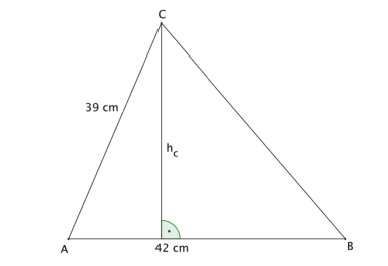
\includegraphics[scale=0.5]{images/A2.1.3.png}
		\end{minipage}
		\begin{enumerate}\setcounter{enumi}{3}
			\item Ein Arbeiter soll eine $5m$ lange Wippe aufstellen. Dazu montiert er am Boden zwei $10cm$ hohe Gummistopper in $4.8m$ Entfernung. Genau zwischen den beiden Stoppern kommt der Standfuss zu stehen, auf dem die Wippe befestigt wird. Wie hoch muss er sein, damit die Schaukelenden auf die Gummis treffen, und wie hoch steigt die Wippe maximal?
			\item Berechne $x,y$ und $z$.\newline
			\begin{minipage}{0.3\linewidth}
				\centering
				\begin{tikzpicture}[cross/.style={draw, cross out, minimum size=2*(#1-1pt), inner sep=0pt, outer sep=0pt}, x=1cm, y=1cm, >=latex,   %Voreinstellung für Pfeilspitzen
					font= \footnotesize, scale=0.6]
					\clip(-2.5,-2.5) rectangle (2.5,2.5);
					\draw (0,0) circle (2cm);
					\draw (0,0) circle (1pt);
					\draw[dashed] (1.73,1) -- (-1.73,-1);
					\draw (-1.73,-1) -- (-1.8,0.87) -- (1.73,1);
					\draw (-1.73,-1) -- (0,-2);
					\draw[color=myblue] (0,-2) -- (1.73,1);
					\draw[color=myblue] (1.2,-0.6) node{$x$};
					\draw (-1.4,0) node {$1.7$};
					\draw (-0.5,-1.25) node {$2.4$};
					\draw (-0.3,1.2) node {$14.4$};
				\end{tikzpicture}
			\end{minipage}
			\hfill
			\begin{minipage}{0.3\linewidth}
				\centering
				\begin{tikzpicture}[cross/.style={draw, cross out, minimum size=2*(#1-1pt), inner sep=0pt, outer sep=0pt}, x=1cm, y=1cm, >=latex,   %Voreinstellung für Pfeilspitzen
					font= \footnotesize, scale=0.6, rotate=70]
					\clip(-2.5,-2.5) rectangle (2.5,2.5);
					\draw (0,0) circle (2cm);
					\draw (0,0) circle (1pt);
					\draw[dashed] (1.73,1) -- (-1.73,-1);
					\draw (-1.73,-1) -- (-1.8,0.87) -- (1.73,1);
					\draw (-1.73,-1) -- (0,-2);
					\draw[color=myblue] (0,-2) -- (1.73,1);
					\draw[color=myblue] (1.2,-0.6) node{$y$};
					\draw (-1.4,0) node {$\sqrt{7}$};
					\draw (-0.4,-1.25) node {$\sqrt{5}$};
					\draw (-0.2,1.5) node {$\sqrt{11}$};
				\end{tikzpicture}
			\end{minipage}
			\hfill
			\begin{minipage}{0.3\linewidth}
				\begin{tikzpicture}[cross/.style={draw, cross out, minimum size=2*(#1-1pt), inner sep=0pt, outer sep=0pt}, x=1cm, y=1cm, >=latex,   %Voreinstellung für Pfeilspitzen
					font= \footnotesize, scale=0.6, rotate=40]
					\clip(-2.5,-2.5) rectangle (2.5,2.5);
					\draw (0,0) circle (2cm);
					\draw (0,0) circle (1pt);
					\draw[dashed] (1.73,1) -- (-1.73,-1);
					\draw[color=myblue] (-1.73,-1) -- (-1.8,0.87);
					\draw (-1.8,0.87) -- (1.73,1);
					\draw (-1.73,-1) -- (0,-2) -- (1.73,1);
					\draw (1.2,-0.6) node{$2$};
					\draw[color=myblue] (-1.4,0) node {$z$};
					\draw (-0.4,-1.25) node {$\frac{3}{2}$};
					\draw (-0.2,1.5) node {$2.4$};
				\end{tikzpicture}
			\end{minipage}
			\item In dieser Aufgabe soll aus den beiden Katheten die Höhe auf die Hypotenuse berechnet werden. Gegeben ist ein rechtwinkliges Dreieck mit $\gamma=90^\circ$, $a=8cm$ und $b=6cm$.
			\begin{enumerate}[label=\alph*)]
				\item Berechne den Flächeninhalt $A$ des Dreiecks sowie die Länge der Hypotenuse $c$.
				\item Berechne nun mithilfe von $A$ und $c$ die Höhe $h_c$.
				\item Stelle allgemein eine Beziehung zwischen $a,b,c$ und $h_c$ auf und bestimme $h_c$.
			\end{enumerate}
		\end{enumerate}
	\end{aufgabe}
	In der Mathematik gilt das Beiweisen als Königsdisziplin. Gleichzeitig ist die Kernkompetenz eines jeden studierten Mathematikers. Jede Aussage soll rigoros bewiesen und begründet werden. Aus diesem Grund wollen wir im folgenden das Schwergewicht auf unterschiedliche Beweise des Satzes von Pythagoras legen. Insgesamt sind über 300 unterschiedliche Beweise bekannt.
	\begin{aufgabe}[Beweis nach Pythagoras und Chou-Pei (ca. 100 v. Chr.)] % Skript Atchu
		Betrachte die folgenden Figuren. Erkläre, wie du damit den Satz des Pythagoras begründen kannst.
		\begin{figure}[H]
			\centering
			\begin{tikzpicture}[cross/.style={draw, cross out, minimum size=2*(#1-1pt), inner sep=0pt, outer sep=0pt}, x=1cm, y=1cm, >=latex,   %Voreinstellung für Pfeilspitzen
				font= \footnotesize, scale=0.22]
				\clip(-27,-1) rectangle (9,15);
				\draw[line width=1pt,color=black,fill=myblue,fill opacity=0.2] (-6,8) -- (0,0) -- (8,6) -- (2,14) -- cycle;
				\draw[line width=1pt,color=black,fill=myblue,fill opacity=0.2] (-26,14) -- (-26,8) -- (-20,8) -- (-20,14) -- cycle;
				\draw[line width=1pt,color=black,fill=myblue,fill opacity=0.2] (-20,8) -- (-20,0) -- (-12,0) -- (-12,8) -- cycle;
				\draw [line width=1pt] (8,14) -- (-6,14);
				\draw [line width=1pt] (-6,14) -- (-6,0);
				\draw [line width=1pt] (-6,0) -- (8,0);
				\draw [line width=1pt] (8,0) -- (8,14);
				\draw [line width=1pt] (-20,14) -- (-12,14);
				\draw [line width=1pt] (-12,14) -- (-12,8);
				\draw [line width=1pt] (-26,8) -- (-26,0);
				\draw [line width=1pt] (-26,0) -- (-20,0);
				\draw [line width=1pt, dashed] (-26,0) -- (-20,8);
				\draw [line width=1pt, dashed] (-20,8) -- (-12,14);
				%rechte Winkel
				\draw [line width=1pt] (8,2) arc[start angle=90,delta angle=90,radius=2cm];
				\draw (7.25,0.75) circle (2pt);
				\draw [line width=1pt] (-12,10) arc[start angle=90,delta angle=90,radius=2cm];
				\draw (-12.75,8.75) circle (2pt);
				\begin{scriptsize}
					\draw[color=black] (4.5,2.5) node {$c$};
					\draw[color=black] (5,-0.5) node {$a$};
					\draw[color=black] (8.5,2.5) node {$b$};
					\draw[color=black] (-16,8.5) node {$a$};
					\draw[color=black] (-11.5,11) node {$b$};
					\draw[color=black] (-16,12) node {$c$};
				\end{scriptsize}
			\end{tikzpicture}
		\end{figure}
		\textbf{Vorgehen bei diesem Beweis:}
		\begin{enumerate}
			\item Begründe, dass die beiden Gesamtfiguren jeweils gleich grosse Quadrate darstellen. Schreibe dazu möglichst viele Streckenlängen an.
			\item Begründe, dass das blaue Viereck im Innern der rechten Figur lauter rechte Winkel besitzt. Es handelt sich also um ein Quadrat.
			\item Wenn es sich zu Beginn also auf beiden Seiten um gleich grosse Figuren handelt, und man auf beiden Seiten je vier identische Dreiecke wegnimmt, muss auch die übrigbleibende Restfläche gleich gross sein. Formuliere diese Tatsache durch eine mathematische Formel.
		\end{enumerate}
		\karos{10}
	\end{aufgabe}
	\begin{aufgabe}[Beweis nach an-Narizi (ca. 900 n. Chr.)]
		Betrachte die folgenden Figuren. Begründe auch damit die Aussage des Satzes von Pythagoras.
		\begin{figure}[H]
			\centering
			\begin{tikzpicture}[cross/.style={draw, cross out, minimum size=2*(#1-1pt), inner sep=0pt, outer sep=0pt}, x=1cm, y=1cm, >=latex,   %Voreinstellung für Pfeilspitzen
				font= \footnotesize, scale=0.18]
				\clip(-34,-2) rectangle (24,24);
				\draw[line width=1pt,color=black,fill=myblue,fill opacity=0.2] (0,6) -- (16,0) -- (22,16) -- (6,22) -- cycle;
				\draw[line width=1pt,color=black,fill=myblue,fill opacity=0.2] (-26,0) -- (-10,0) -- (-10,16) -- (-26,16) -- cycle;
				\draw[line width=1pt,color=black,fill=myblue,fill opacity=0.2] (-32,0) -- (-26,0) -- (-26,6) -- (-32,6) -- cycle;
				\draw [line width=1pt] (0,6) -- (0,0);
				\draw [line width=1pt] (0,0) -- (22,0);
				\draw [line width=1pt] (22,0) -- (22,16);
				\draw [line width=1pt, dashed] (0,6) -- (6,6);
				\draw [line width=1pt, dashed] (22,16) -- (6,16);
				\draw [line width=1pt, dashed] (6,22) -- (6,3.75);
				%rechte Winkel
				\draw [line width=1pt] (2,0) arc[start angle=0,delta angle=90,radius=2cm];
				\draw (0.75,0.75) circle (2pt);
				\draw [line width=1pt] (22,2) arc[start angle=90,delta angle=90,radius=2cm];
				\draw (21.25,0.75) circle (2pt);
				\begin{scriptsize}
					\draw (-18,-1) node {$b$};
					\draw (-9,8) node {$b$};
					\draw (-28,-1) node {$a$};
					\draw (-33,3) node {$a$};
					\draw (8,-1) node {$b$};
					\draw (19,-1) node {$a$};
					\draw (-1,3) node {$a$};
					\draw (23,8) node {$b$};
				\end{scriptsize}
			\end{tikzpicture}
		\end{figure}
		\textbf{Vorgehen bei diesem Beweis:}
		\begin{enumerate}
			\item Begründe, dass das blaue Viereck in der rechten Figur ein Quadrat ist.
			\item Begründe mit eigenen Worten, warum die beiden blauen Flächen gleich gross sind.
			\item Erkläre, wie du daraus den Satz des Pythagoras formulieren kannst.
		\end{enumerate}
		\karos{14}
	\end{aufgabe}
	\begin{aufgabe}[Beweis nach Garfield (ca. 1850)] % Skript Atchu
		Betrachte die folgenden Figuren. Begründe auch damit die Aussage des Satzes von Pythagoras.
		\begin{figure}[H]
			\centering
			\begin{tikzpicture}[cross/.style={draw, cross out, minimum size=2*(#1-1pt), inner sep=0pt, outer sep=0pt}, x=1cm, y=1cm, >=latex,   %Voreinstellung für Pfeilspitzen
				font=\footnotesize, scale=0.2]
				\clip(-2,-2) rectangle (18,23);
				\draw [line width=1pt] (0,22) -- (6,22);
				\draw [line width=1pt] (6,22) -- (0,6);
				\draw [line width=1pt] (0,6) -- (0,22);
				\draw [line width=1pt] (0,6) -- (0,0);
				\draw [line width=1pt] (0,0) -- (16,0);
				\draw [line width=1pt] (16,0) -- (0,6);
				\draw [line width=1pt] (6,22) -- (16,0);
				\draw [line width=1pt] (1.87,5.3) arc[start angle=-20.56,delta angle=90,radius=2cm];
				%Rechte Winkel
				\draw [line width=1pt] (2,0) arc[start angle=0,delta angle=90,radius=2cm];
				\draw (0.75,0.75) circle (2pt);
				\draw [line width=1pt] (0,20) arc[start angle=270,delta angle=90,radius=2cm];
				\draw (0.75,21.25) circle (2pt);
				\begin{scriptsize}
					\draw (2.5,7) node {$\gamma$};
					\draw (-1,4) node {$a$};
					\draw (8,-1) node {$b$};
					\draw (8,4) node {$c$};
				\end{scriptsize}
			\end{tikzpicture}
		\end{figure}
		\textbf{Vorgehen bei diesem Beweis:}
		\begin{enumerate}
			\item Zeige, dass $\gamma=90^\circ$.
			\item Berechne den Flächeninhalt des entstehenden Trapezes auf zwei verschiedene Arten (einerseits besteht die Figur aus drei Dreiecken, andererseits handelt es sich eben um ein Trapez: entweder kannst Du Dich noch an die Flächenformel für Trapeze erinnern, oder Du findest einen anderen Weg).
			\item Wenn Du diese beiden Resultate miteinander vergleichst, müsstest Du einen Beweis des Satzes von Pythagoras erkennen.
		\end{enumerate}
		\karos{10}
	\end{aufgabe}\newpage




\section{Anwendungen von Pythagoras}
\subsection{Die Raumdiagonale}
	\begin{beispiel}\ \vspace{5pt}\newline
		\begin{minipage}{0.475\linewidth}
			Peter möchte seinem Onkel per Post einen $135cm$ langen Stab schicken. Zu Hause liegt eine Schachtel mit den Kantenlängen $a=100$ cm, $b=80$ cm und $c=60$ cm herum. Passt der Stab vollständig in diese Schachtel? \\
			\textit{Der Stab ist sehr dünn. Die Dicke des Stabes muss für unsere Überlegungen also nicht berücksichtigt werden.}
		\end{minipage}
		\hfill
		\begin{minipage}{0.475\linewidth}
			\centering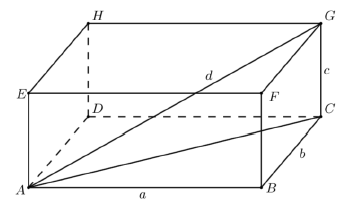
\includegraphics[scale=0.8]{images/raumdiagonale.png}
		\end{minipage}
	\end{beispiel}
	\begin{definition}
		Die Raumdiagonale eines Quaders ist der Abstand zwischen zwei möglichst weit voneinander entfernten Punkten des Quaders.
	\end{definition}
	Im oben dargestellten Quaders sind die Strecken $\overline{AG}$, $\overline{BH}$, $\overline{CE}$ und $\overline{DF}$ die Raumdiagonalen.\newline
	Wie können wir aber die Länge dieser Raumdiagonalen berechnen?\vspace{5pt}\newline\karos{6}
	Als Folge deiner Berechnungen können wir also folgende Formel festhalten:
	\begin{satz}
		Die Raumdiagonale $d$ eines Quaders mit den Kantenlängen $a,b$ und $c$ hat die Länge \[d=\gap{4}.\]
	\end{satz}
	Wir können nun also berechnen, ob Peters Stab in seine Kiste passt.\vspace{5pt}\newline\karos{3}
	\begin{aufgabe}
		\begin{enumerate}
			\item Berechne die eingezeichneten Grössen.\newline
			\begin{minipage}{0.457\linewidth}
				\centering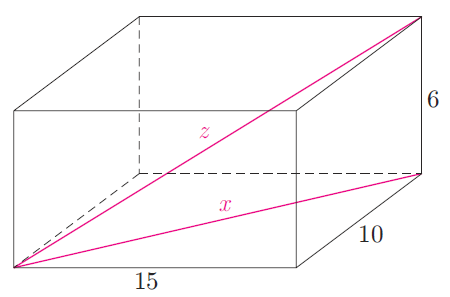
\includegraphics[scale=0.5]{images/A2.5.1.png}
			\end{minipage}
			\hfill
			\begin{minipage}{0.475\linewidth}
				\centering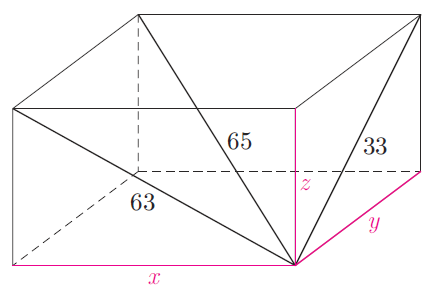
\includegraphics[scale=0.5]{images/A2.5.2.png}
			\end{minipage}
			\item Timmy möchte ein Schwimmabzeichen erhalten. Dafür muss er $16m$ tauchen können. Er befindet sich in einem $10m$ breiten, $28m$ langen und $2m$ tiefen Schwimmbecken. Er schwimmt zur Beckenmitte. Dort taucht er hinunter zum Beckengrund, holt einen Tauchring und setzt seinen Tauchgang auf direktem Weg zu einer Ecke an der Oberfläche fort. Hat er die erforderliche Länge geschafft?
		\end{enumerate}
	\end{aufgabe}


\subsection{Die Höhe im gleichseitigen Dreieck}
	\begin{beispiel}\ \newline
		\begin{minipage}{0.6\linewidth}
			Jedes gleichseitige Dreieck ist achsensymmetrisch, kann also durch die Höhe in zwei kongruente, rechtwinklige Dreieck zerlegt werden.
			Berechne die Höhe $h$ für ein gleichseitiges Dreieck...
			\begin{enumerate}[label=\alph*)]
				\item mit Seitenlänge $s=8cm$.
				\item mit allgemeiner Seitenlänge $s$
			\end{enumerate}
		\end{minipage}
		\hfill
		\begin{minipage}{0.35\linewidth}
			\centering
			\begin{tikzpicture}[cross/.style={draw, cross out, minimum size=2*(#1-1pt), inner sep=0pt, outer sep=0pt}, x=1cm, y=1cm, >=latex,   %Voreinstellung für Pfeilspitzen
				font=\footnotesize, scale=0.5]
				\clip(-6,-2) rectangle (6,7);
				\draw[line width=1pt] (-4,0) -- (4,0) -- (0,6) -- cycle;
				\draw[line width=1pt] (0,6) -- (0,0);
				%Rechte Winkel
				\draw [line width=1pt] (1,0) arc[start angle=0,delta angle=90,radius=1cm];
				\filldraw (0.4,0.4) circle (2pt);
				\begin{scriptsize}
					\draw (2.5,3) node {$s$};
					\draw (-2.5,3) node {$s$};
					\draw (2.5,-0.75) node {$\frac{s}{2}$};
					\draw (-2.5,-0.75) node {$\frac{s}{2}$};
					\draw (0.5,2.5) node {$h$};
					\draw (-4.5,-0.2) node {$A$};
					\draw (4.5,-0.2) node {$B$};
					\draw (0.2,6.5) node {$C$};
				\end{scriptsize}
			\end{tikzpicture}
		\end{minipage}
		\vspace{5pt}\karos{8}
	\end{beispiel}
	\begin{satz}
		Die Länge $h$ der Höhe eines gleichseitigen Dreiecks mit Seitenlänge $s$ beträgt \[h=\gap{4}.\]
	\end{satz}
	\begin{aufgabe}
		tbd
	\end{aufgabe}

\subsection{Der Kathetensatz}

\subsection{Der Höhensatz}

\subsection{Die Flächenformel nach Heron}


\newpage
\subsection*{History}
\begin{table}[H]
	\centering
	\begin{tabular}{|p{13mm}|p{20mm}|p{30mm}|p{70mm}|}\hline
		%\multicolumn{4}{|l|}{History}\\\hline
		Version & Datum & Person & Bemerkung \\\hline
		$1.0$ & 08.12.24 & Jonas Guler & Abschnitt 1\&2 erstellt \\\hline
		$1.1$ & ToDo & Jonas Guler & Abschnitt 3 ergänzen \\\hline
	\end{tabular}
\end{table}

\end{document}